\chapter{Week 5: Data analyse in Python}

We hebben inmiddels een gedegen bassis kennis van \textit{Python} opgedaan gedurende dit vak. We hebben o.a. geleerd over loops, lijsten, functies en IO aansturing in \textit{Python}, en de vershillen gezien met \textit{C}. Een van de concepten die nog onbelicht is gebleven is het zogeheten 'object georiënteerd programmeren' (of \textit{OOP}).
Omdat dit een van de belangrijkste en handigste concepten van het programmeren is van de afgelopen decenia, én omdat we stiekem er toch al flink mee gewerkt hebben, gaan we in dit hoofdstuk ook dit thema belichten. Daarnaast gaan we deze week aan de slag met \textit{packages}, handige software bibliotheken die de functionaliteit van onze \textit{Python} omgeving kunnen uitbreiden. 

\section{Object georiënteerd programmeren}\index{Object georiënteerd programmeren}


\section{Packages}\index{Packages}
Een \textit{Package} in \textit{Python} is een verzameling van modules. Deze modules kunnen we weer in onze code gebruiken door deze te importeren met \pyth{import}. We hbben er in middel al een aantal van gebruikt bijv.: \pyth{math, time, gpiozero, RPi.GPIO}, maar deze worden allemaal standaard meegeleverd. Je kunt ze ook heel eenvoudig zelf toevoegen aan je \textit{Python} omgeving, door gebruik te maken van \pyth{pip}. Dit programma kun je aanroepen vanaf de terminal:
\begin{lstlisting}[language=bash]
python3 -m pip install <naam_package>
\end{lstlisting}

\begin{remark}
  Je hebt ongetwijfeld al een hele lijst geïnstalleerd zonder dat je het wist, je kunt het bekijken door het onderstaande in een terminal in te typen: 
  \begin{lstlisting}[language=bash]
  python3 -m pip list
  \end{lstlisting}
\end{remark}

Om een beetje bekend te raken met \textit{pip}, gaan we als voorbeeld een kleine package installeren genaamd \pyth{camelcase}:
\begin{lstlisting}[language=bash]
python3 -m pip install camelcase
\end{lstlisting}

Probeer nu het volgende scriptje te draaien:
\begin{python}
from camelcase import CamelCase     # importeer onze nieuwe aanwinst

c = CamelCase()                     # Nodig om de package te kunnen gebruiken.
txt = 'pip onder de knie krijgen!'  # De tekst die omgezet dient te woren.

print(c.hump(txt))                  # Pas camelcase toe op de tekst.
\end{python}
Als dat lukt, is de module juist geïnstalleerd en heb je de basis van \textit{pip} onder de knie! (Deze packages worden overigens gedownload vanaf \url{https://pypi.org/}, kijk er gerust eens na en wellicht kom je er interressante tegen tussen de bijna 350.000 packages.) \\
Het aanpassen van hoofdletters is echter niet al te spannend, dus gaan we verder met een package waar we echt iets aan hebben: \textit{matplotlib}. 
\begin{exercise}
  Installeer Matplotlib
\end{exercise}

Matplotlib is een verzameling aan tools voor het maken en bewerken van grafieken. Om het te gebruiken in z'n meest simpele vorm zorg je ervoor dat je een reeks $x$-waardes hebt, en een reeks bijbehorende $y$-waardes. Deze kun je dan plotten (het daadwerkelijk tekenen van de grafiek) en de resulterende grafiek kun je tonen op het scherm.

\begin{python}
import matplotlib.pyplot as plt

# Creeer x en y waardes ahv lijsten:
x = [0,1,2,3,4,5,6,7,8,9] 
y = [2,3,4,5,1,2,3,4,7,1]

# Plot de waardes, en laat hierna de grafiek zien:
plt.plot(x, y)
plt.show()
\end{python}

Hieruit rolt de de grafiek uit \ref{fig:plot1}:
\begin{figure}[h!]
\centering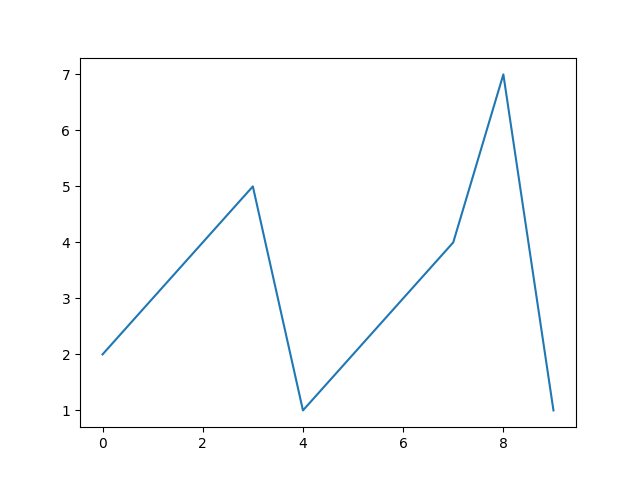
\includegraphics[scale=0.7]{Pictures/chapter07/plot1.png}
\caption{Simpele plot met \textit{Matplotlib}}
\label{fig:plot1} % Unique label used for referencing the figure in-text
%\addcontentsline{toc}{figure}{Figure \ref{fig:webserver}} % Uncomment to add the figure to the table of contents
\end{figure}

\begin{remark}
Kreeg je bij het runnen van bovenstaande code op de \textit{Pi} een error, in de trant van \textit{'Error retrieving accessibility bus address'}? Dan kan het zijn dat je een module in Linux mist, open een terminal en voer in: 
\begin{lstlisting}[language=bash]
sudo apt-get update
sudo apt-get install at-spi2-core
\end{lstlisting}
\end{remark}


\inputpython{code/chapter07/plot1.py}{1}{24}


  

% \subsection{pip}\index{pip}

% \section{CSV file edit}\index{CSV file edit}
% \subsection{Excel file edit}\index{Excel file edit}

% \section{Matplotlib}\index{Matplotlib}

% \newpage

% \section{Opdrachten}\index{Opdrachten}
% \begin{exercise}
% $\\$
% \end{exercise}

% \begin{exercise}
% $\\$
% \end{exercise}

% \begin{exercise}
% $\\$
% \end{exercise}

% \begin{exercise}
% $\\$
% \end{exercise}

% \begin{exercise}
% $\\$
% \end{exercise}

% \begin{exercise}
% $\\$
% \end{exercise}

% \begin{exercise}
% $\\$
% \end{exercise}

% \begin{exercise}
% $\\$
% \end{exercise}

